\section{РЕАЛИЗАЦИЯ И ИСПОЛЬЗОВАНИЕ}
\label{sec:manual}

После изучения иструментов разработки и построенной архетектуре осталось реализовать сервиса управления серверами.
В данной работе реализованы серверная и клиентская часть приложения. Создание серверной части включает следующие
задачи:
\begin{itemize}
  \item создание API для возможности взаимодействия клиента с сервером;
  \item создание внутренних функций для получения информации для графических элементов представления информации;
  \item создание внутренних функций для взаимодействи с сервером клиент;
  \item создание веб-сокет соединений с клиентом.
\end{itemize}


Также стоит упомянуть про реализацию клиента. Создание клиентской части включало следующие задачи:
\begin{itemize}
\item реализация взаимодействия с API сервера;
\item реализация взаимодействия с пользователем;
\item построение графиков и графических представления спомощью d3;
\item работа в веб-сокетами.
\end{itemize}

Первый пункт включает получение и обработку информации с сервера. Второй – реализацию пользовательских интерфейсов, включая верстку, создание функционального дизайна. В третьем пункте происходит взаимодействие с
данными с сервера и пользователем, строятся графики с помощью библиотеки d3.js. В четвертом также происходит взаимодействие с данными с сервера и пользователем, но через веб-сокет соединение.

\subsection{Руководство пользователя}

Рассмотри функционал и возможности сервиса.

После того как пользователь авторизировался он видит гравную страницу (рисунок 7.1). Страница представляет собой секцию с навигацией по странице и главную секцию, на которой расположен оснойвной контент приложения.

На странице евентов можно видеть события, которые происходят на серверах клиетов. Эти события приходят в реальном времени и хранятся в базе. Так что пользователь может просмотреть все события. Это отличный способ для логирования всех процессов и своевременного ответа на ошибки. Каждое событие имеет свой тип (ok, fatal, warning). События визуально отличаются в зависимости от их типа. 

\begin{figure}[h!]
\centering
	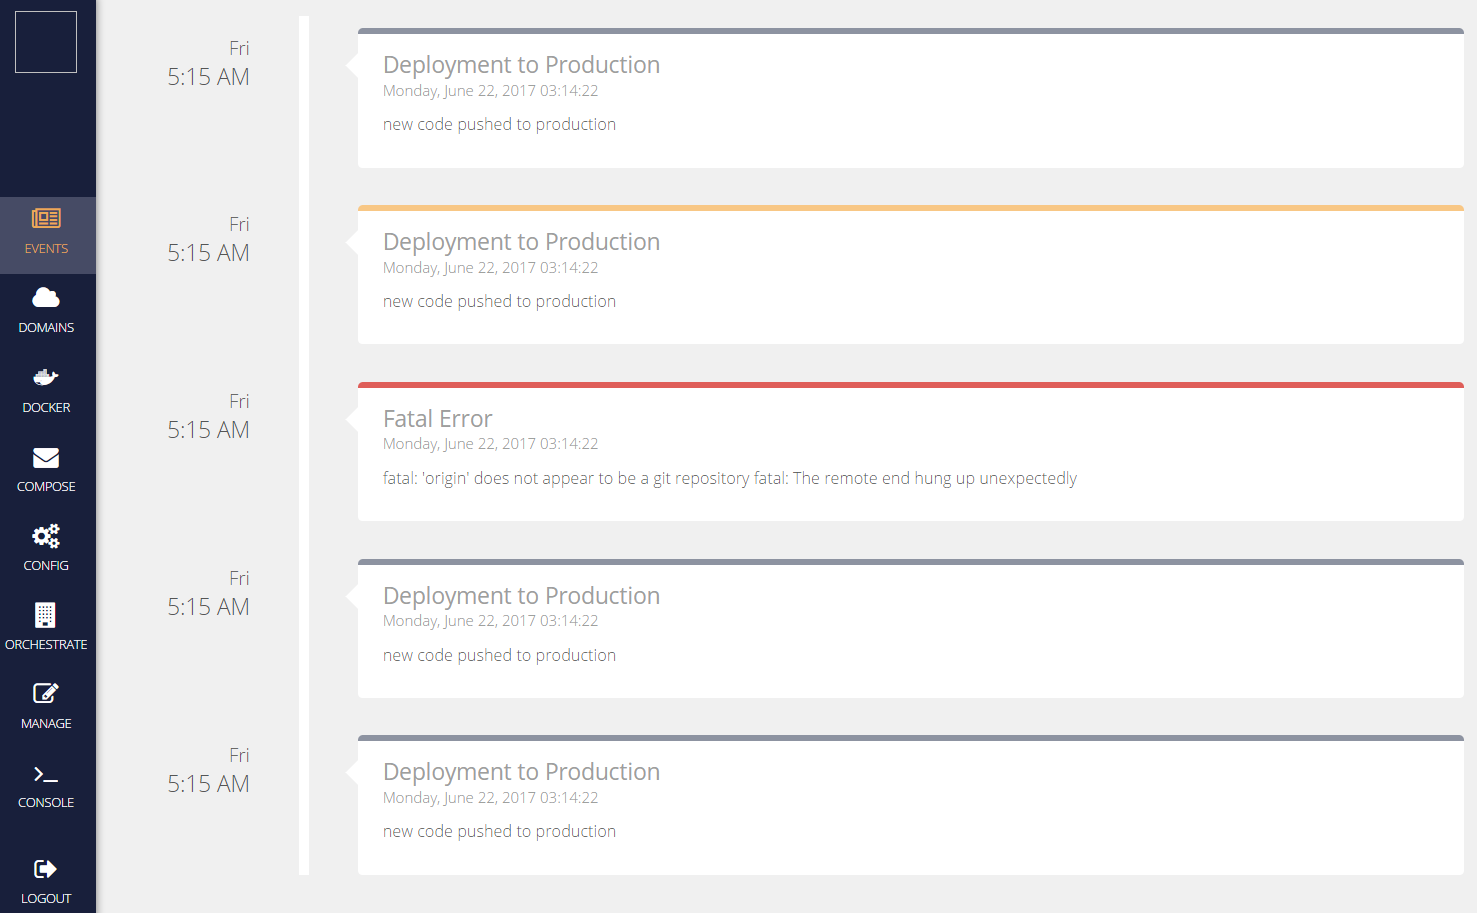
\includegraphics[scale=0.5]{event.png}
	\caption{Страница с евентами}
	\clearpage
\end{figure}

Страница <<Domains>> предназначена для пердставления разных параметров серверов. Для начала пользователю предоставляется возможность выбрать интересующее решение (рисунок 7.2). \linebreak

\begin{figure}[h!]
\centering
	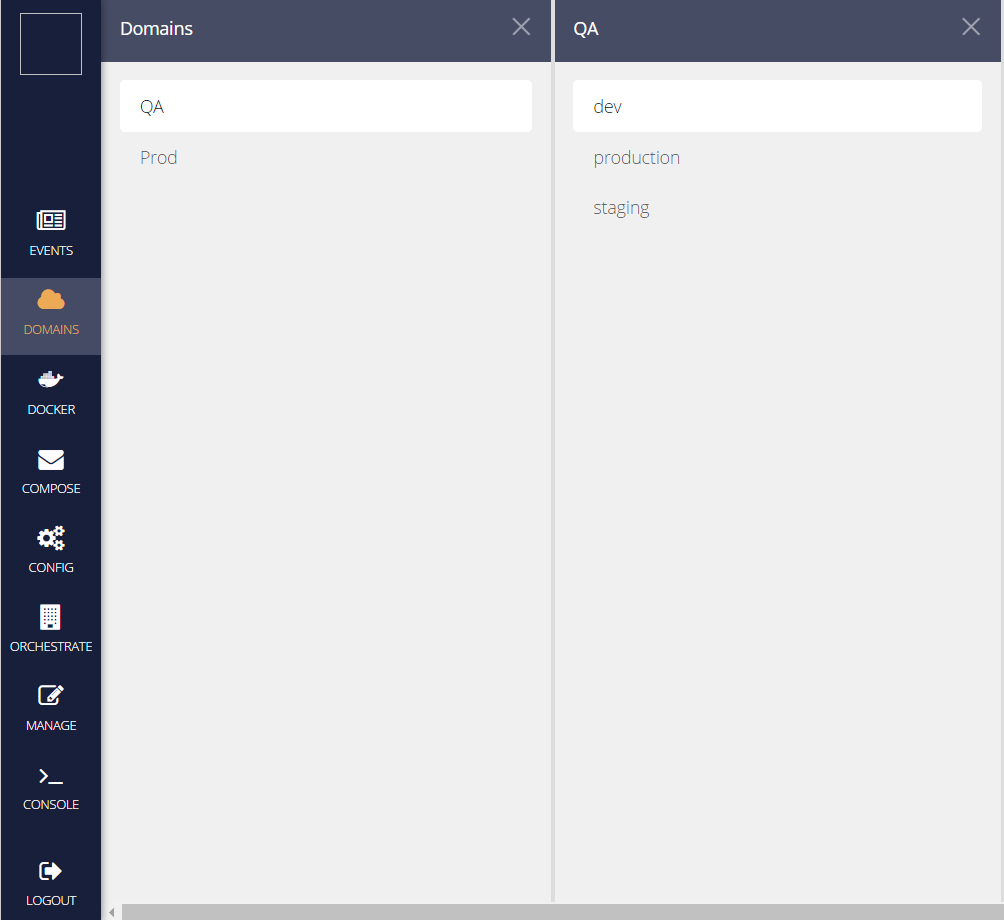
\includegraphics[scale=0.5]{domains-1.png}
	\caption{Навигация на странице domains}
	\clearpage
\end{figure}

Нужно выбрать проект, а потом и нужною ветку этого проета. После выбора появляется основная информация о системе (рисунок 7.3). Весь контент разделён на три части. На одной — информация о самостоятельных сервисах, которые использует клиент, например nginx и redis. На второй — логи приложения, как на главной странице, но уже только для выбраной системы. И третья часть представлена кнопками для перехода на информацию о структуре системы, о используемых ресурсах и о трафике.

\begin{figure}[h!]
\centering
	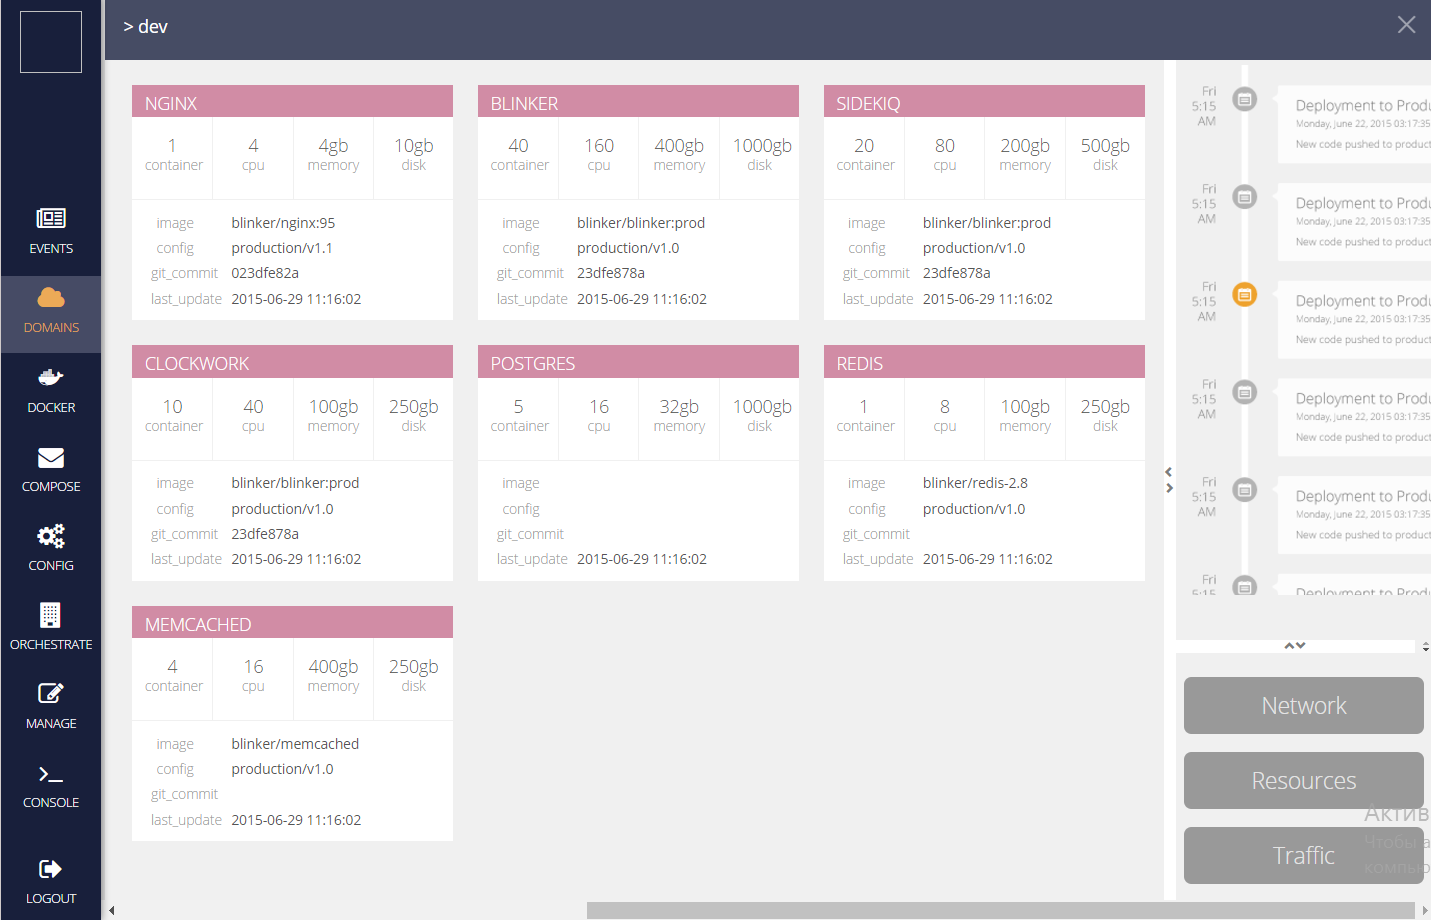
\includegraphics[scale=0.5]{domains-2.png}
	\caption{Основная информация}
	\clearpage
\end{figure}

Рассмотрим все виды схематического представления. Страница <<Network>> впедставляет схематичную структуру системы (рисунок 7.4). Т.е. есть главный сервер и дочерние. 

\begin{figure}[h!]
\centering
	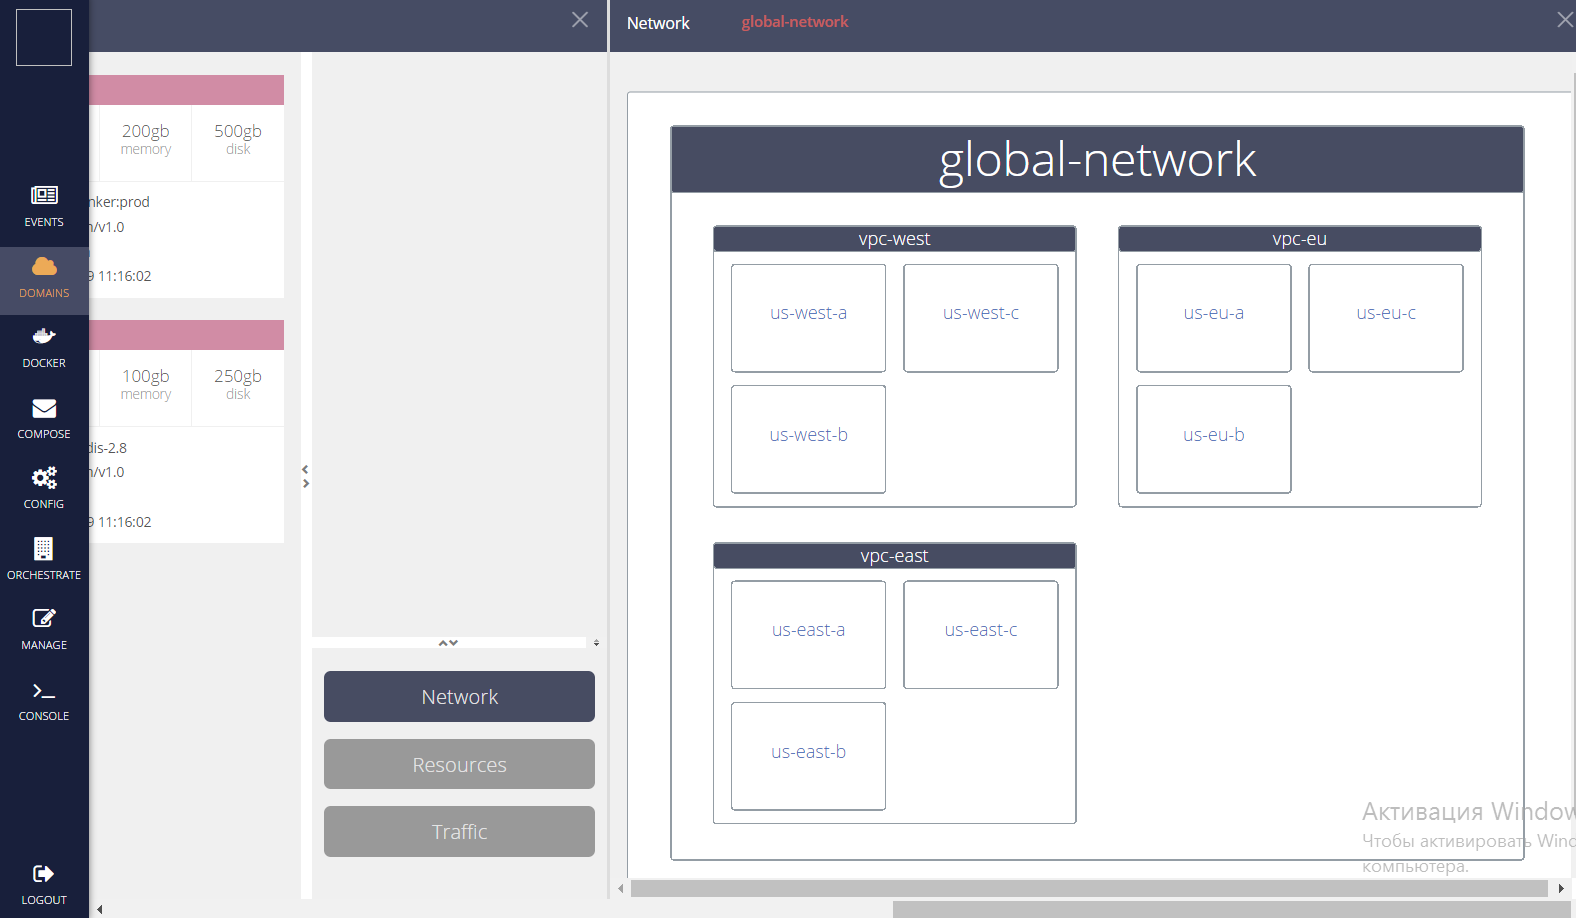
\includegraphics[scale=0.5]{domains-3.png}
	\caption{Схематичная структура системы}
	\clearpage
\end{figure}

Главный сервер представлен большим прямоугольником, а дочерние включены в главный. Это визуализация похожа на карту. Т.е. можно скролить эту область. Элементы схемы становятся больше и появляются дочерние элементы. Так же, как и карту, можно драгать и перемещаться по области (рисунок 7.5). При нажатии на элемент, он цетрируется по области. 

\begin{figure}[h!]
\centering
	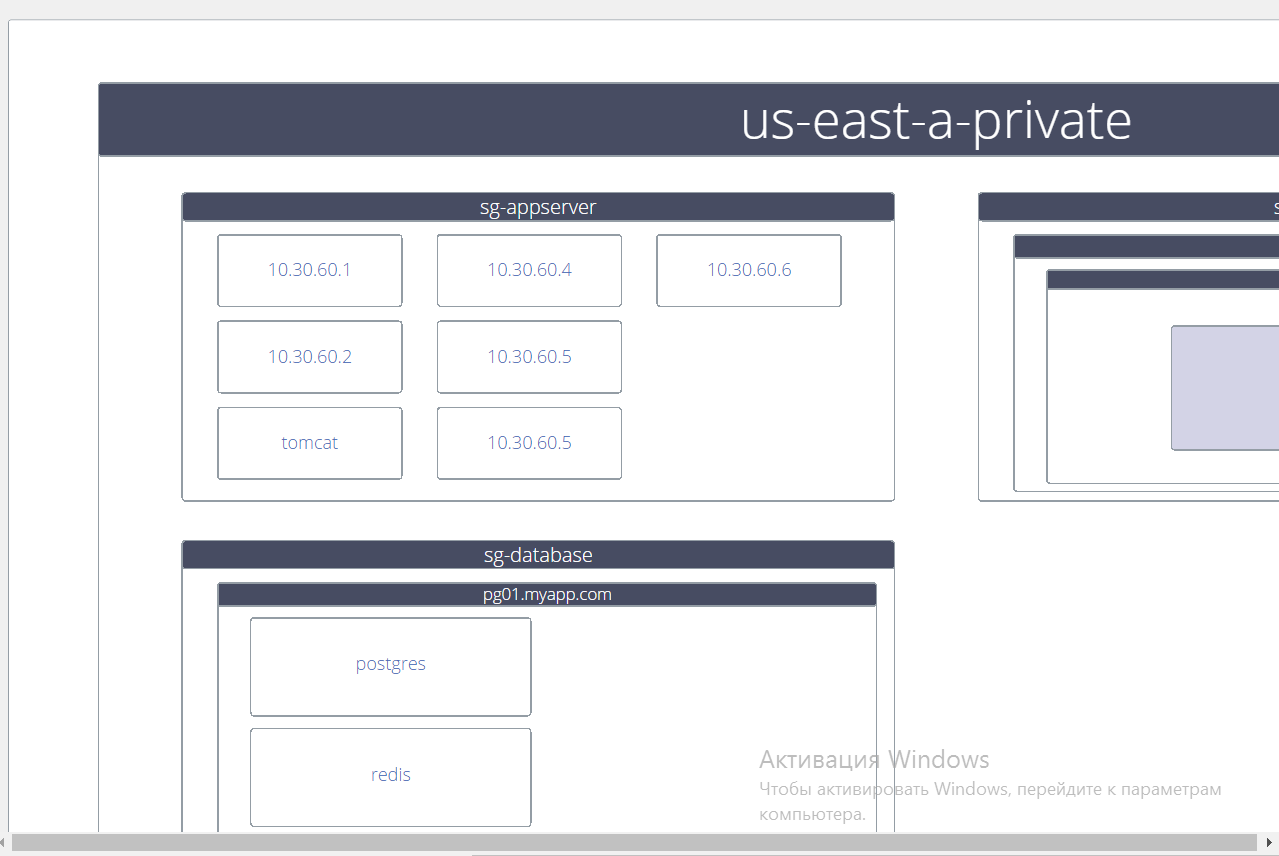
\includegraphics[scale=0.5]{domains-4.png}
	\caption{}
	\clearpage
\end{figure}

Страница Resources представлена прямоугольниками (рисунок 7.6). Елементы имеют разный цвет в зависимости от сервиса. На странице есть два селекта. В зависимости от них меняются расположение и порядок элементов. В селектах можно сортировать по названию, сервису, загрузке цп, количеству. 

\begin{figure}[h!]
\centering
	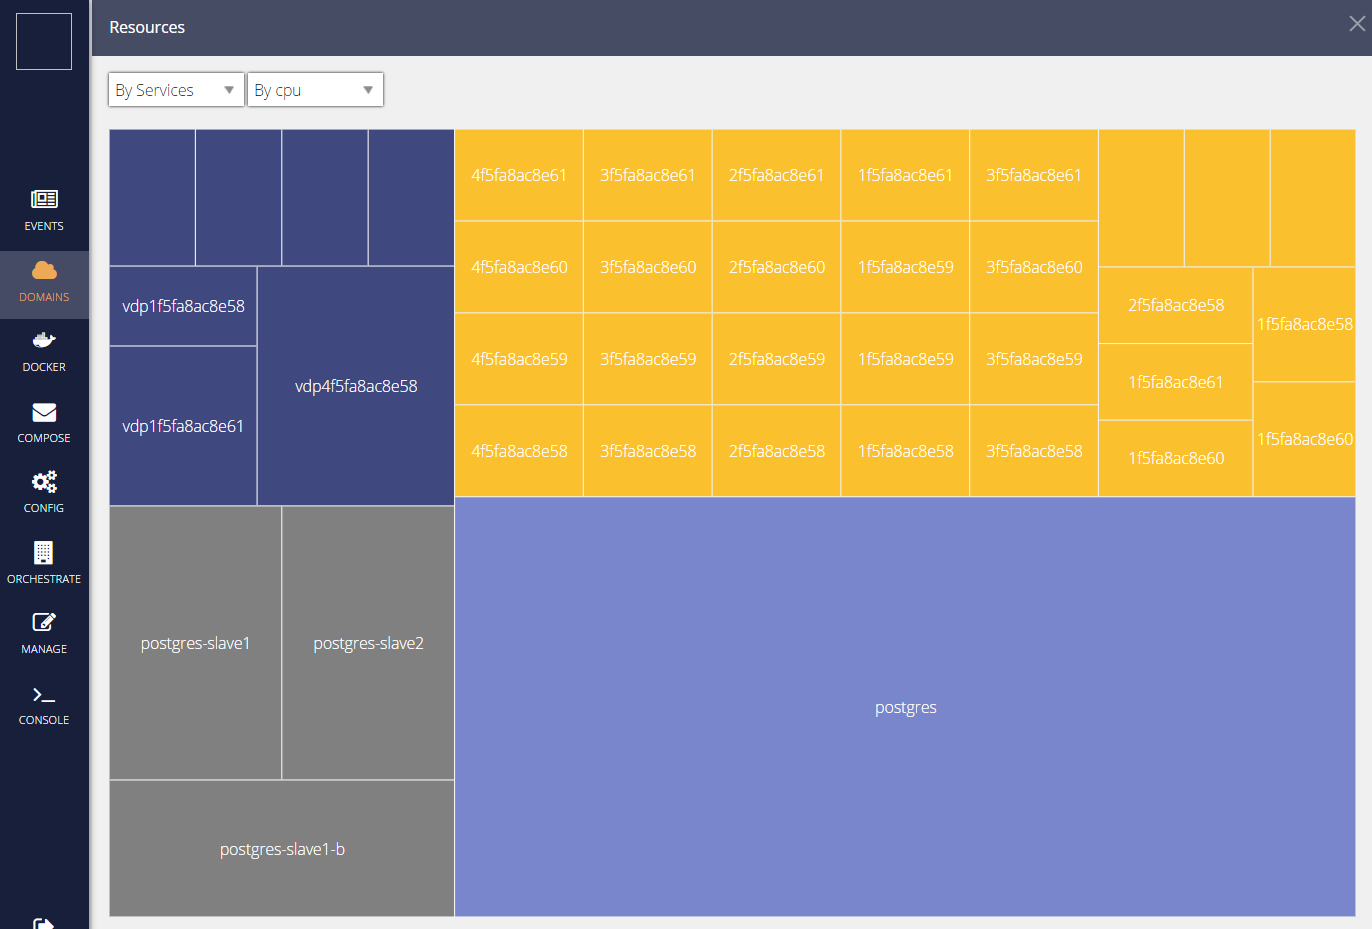
\includegraphics[scale=0.5]{domains-5.png}
	\caption{Ресурсная структура системы}
	\clearpage
\end{figure}

В этих визуализациях используется очень мощная библиотека d3. Она позволяет очень быстро работать с большими массивами данных. Часто используется для визуализации в области bigData.

Страница <<Docker>> предназначена для предоставления информации от сервиса docker. Там есть абсолютно все и почти всегда к продукту приложена инструкция по развертыванию с примерами и описаниями особенностей запуска. Вместо того, чтобы читать многостраничный мануал по установке и настройке продукта, запускаем 1-2 команды, снесли, и следов в системе не остается. 

В блоке <<Summary>> изображается общая информация о docker (рисунок 7.7). Есть возможность посмотреть графики времени создания container и image, статус container и работающие container.

\begin{figure}[h!]
\centering
	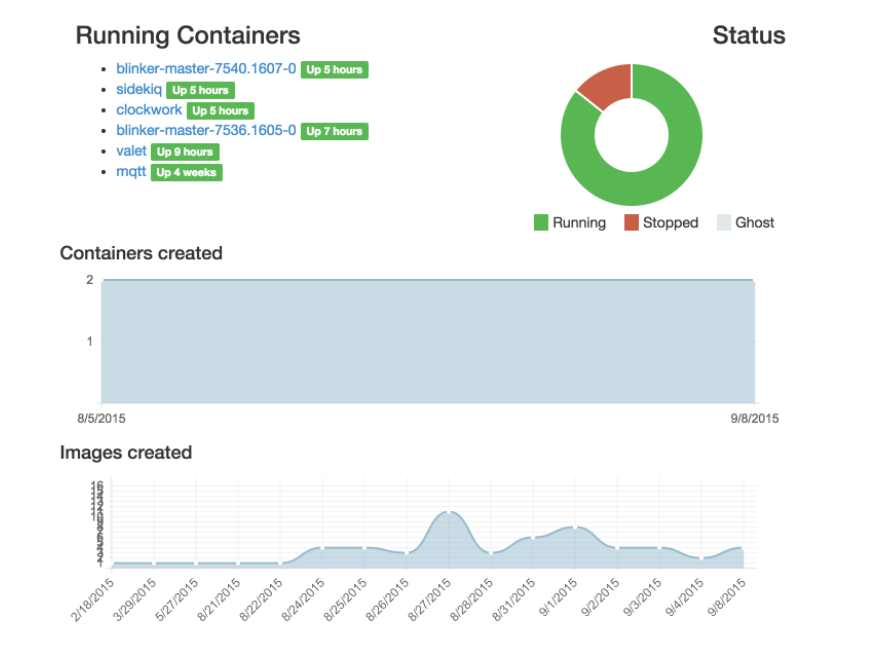
\includegraphics[scale=0.8]{domains-6.png}
	\caption{Общая информация о Docker}
	\clearpage
\end{figure}

Блоки <<Container>> и <<Image>> показывают более подробную информацию. Для примера можно показать только для container. Блок Image имеют такую же структуру. Есть фильтр для поиска элементов.

\begin{figure}[h!]
\centering
	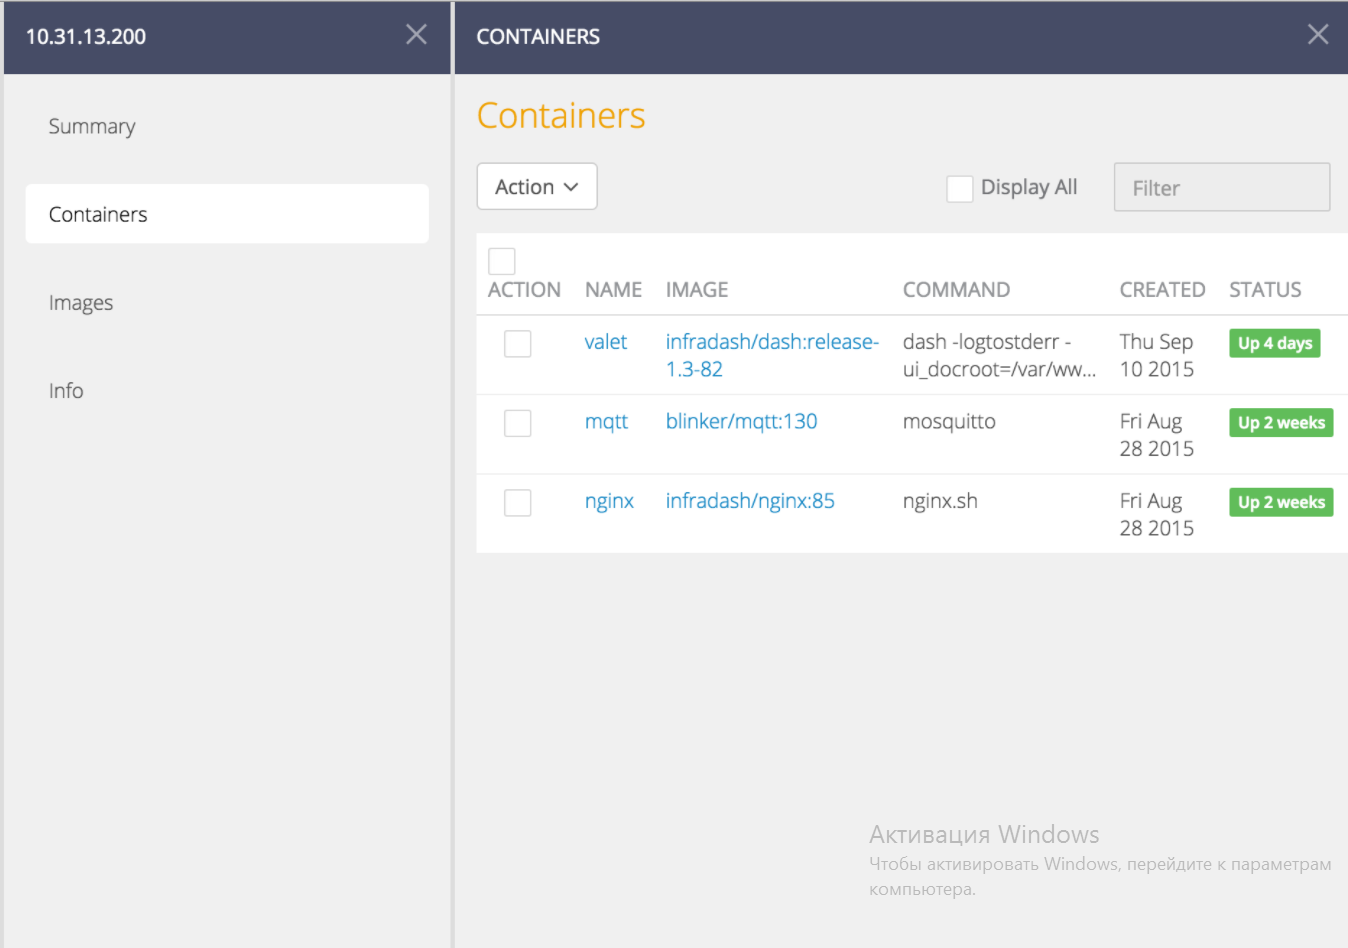
\includegraphics[scale=0.5]{docker-2.png}
	\caption{Информация о Container}
	\clearpage
\end{figure}

Страница <<Config>> предназначена для взаимодействия с конфигами, переменными окружения и пакетами. Для начала предоставляется возможность выбрать раздел <<Configuration files>>, <<Enviroment variables>> или <<Packages>>. При переходе по первой вкладке появляется спосок существующих конфигов, а так же кнопка для создания нового конфига (рисунок 7.9). После нажатия на кнопку <<Add new>> появляется модальное окно, где можно ввести название конфигурационного файла и ввести текст самого файла. После нажатия на конфиг открывается текст конфига (рисунок 7.10). 

\begin{figure}[h!]
\centering
	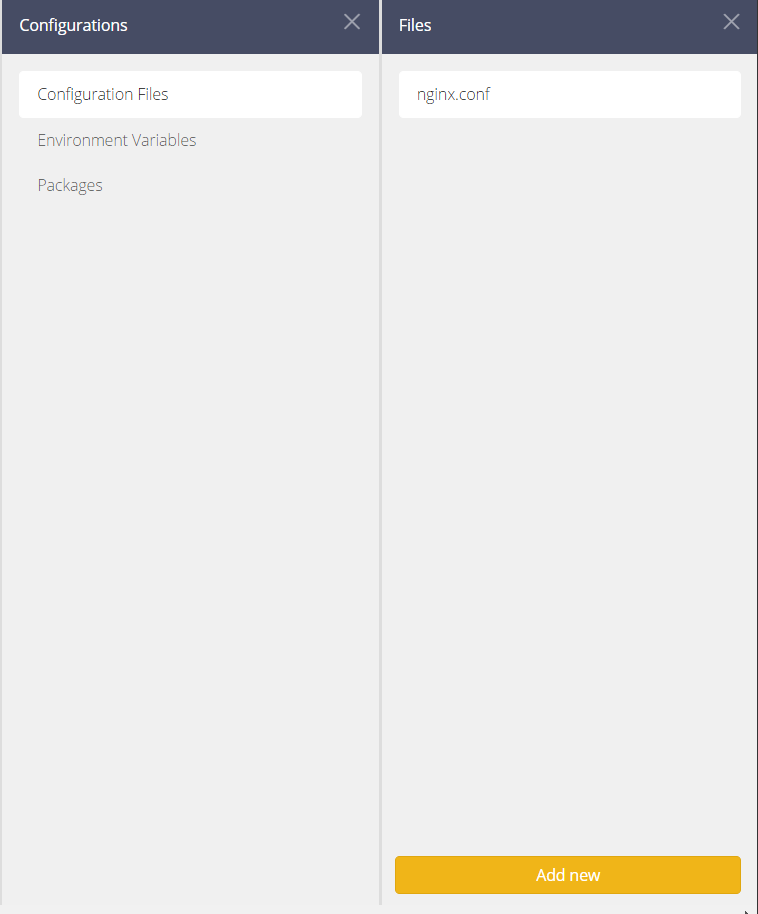
\includegraphics[scale=0.6]{config-1.png}
	\caption{Конфигурационные файлы}
	\clearpage
\end{figure}

Открытое окно предоставляет возможность отредактировать и сохранить и изменения. Есть два селекта, которые позволяют изменять ветку и версию, изменяя тем самым конфиг в редакторе. 

\begin{figure}[h!]
\centering
	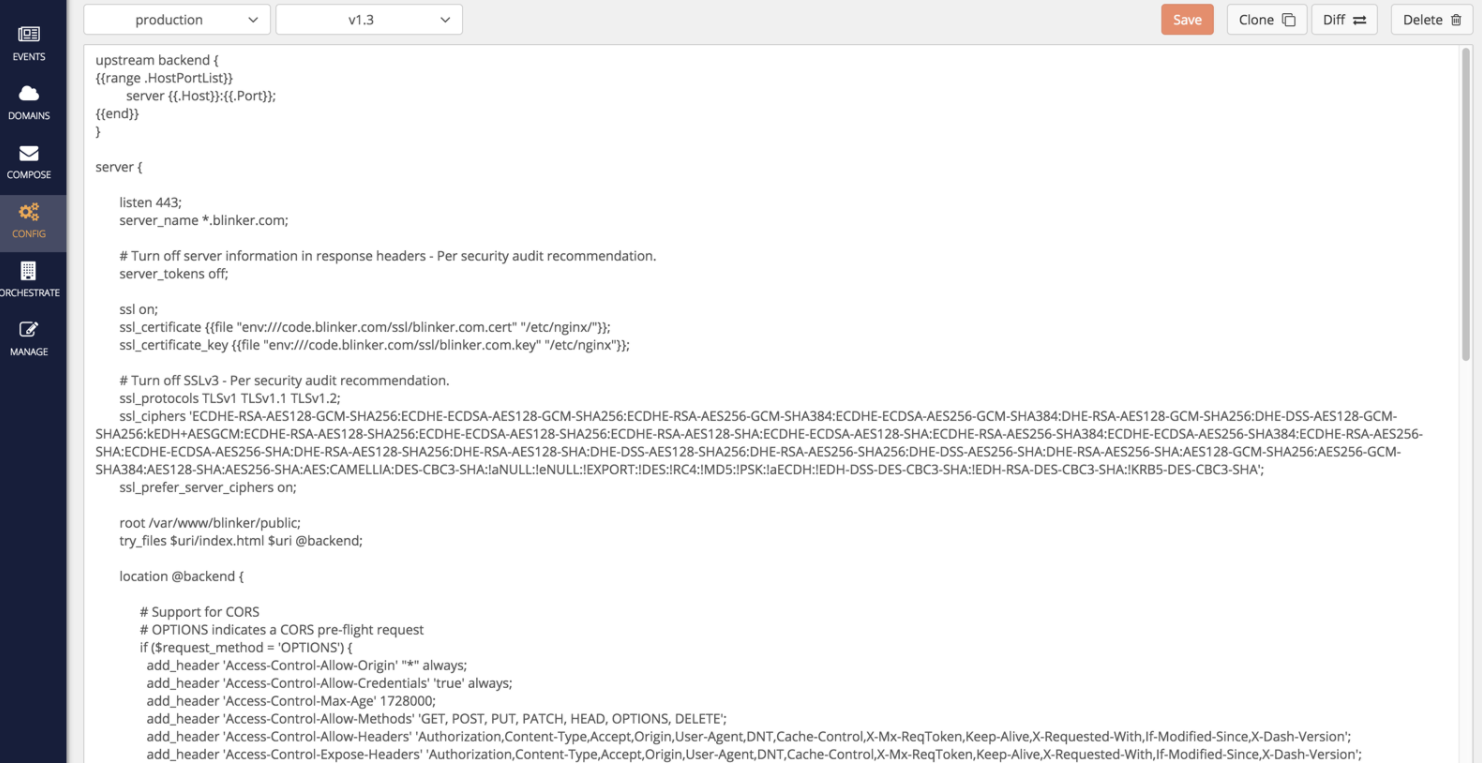
\includegraphics[scale=0.55]{config-2.png}
	\caption{Открытый конфиг}
	\clearpage
\end{figure}

При перехоже на вкладку <<Enviroment variables>> появляются все переменные окружения. Для подробного просмотра можно выбрать только интересующие переменный спомощью чекбоксов. После начатия на кнопку <<Show>> появляется таблица с выбранными переменными (рисунок 7.11). В первом столбике расположены название переменных, а в строчке их значения в зависимости от версии и ветки. Если нет такой переменной, то прямоугольник будет красным. Здесь же можно задать и изменить переменную.

\begin{figure}[h!]
\centering
	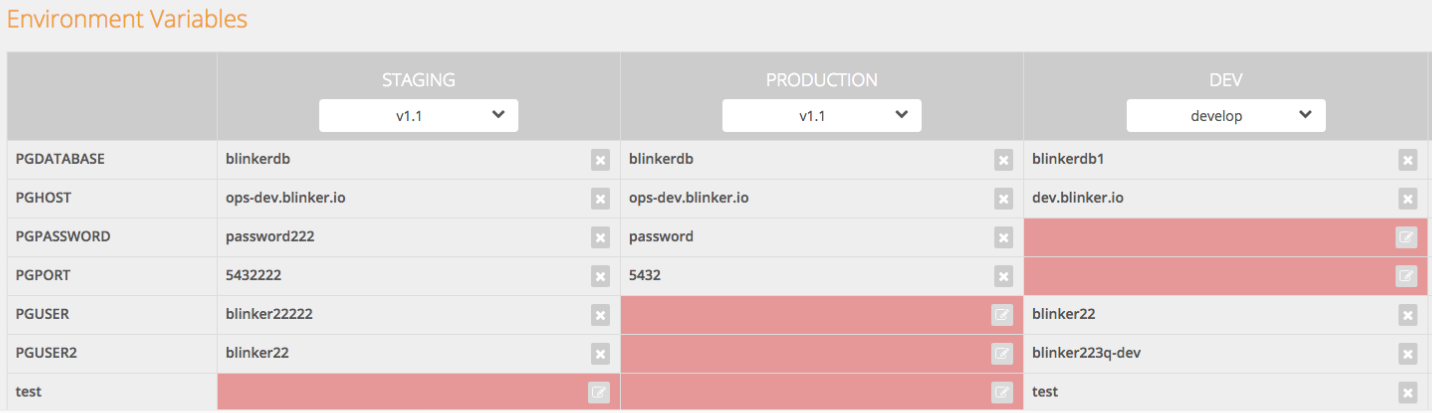
\includegraphics[scale=0.45]{config-3.png}
	\caption{Открытые переменные}
	\clearpage
\end{figure}

Вкладка <<Packages>> имет такой же интерфейс и функционал как и вкладка <<Enviroment variables>>.

На странице <<Manage>> показаны все пользователи, которые имеют совмесный доступ к проектам (рисунок 7.12). У каждого пользователя есть скоуп прав, с комощью которых он может взаимодействовать с проектами. Т.е. может ли он изменять что-то в проекте или его мозможности ограничены только просмотром информации. Это защитит проет от нежелательных изменений.  

\begin{figure}[h!]
\centering
	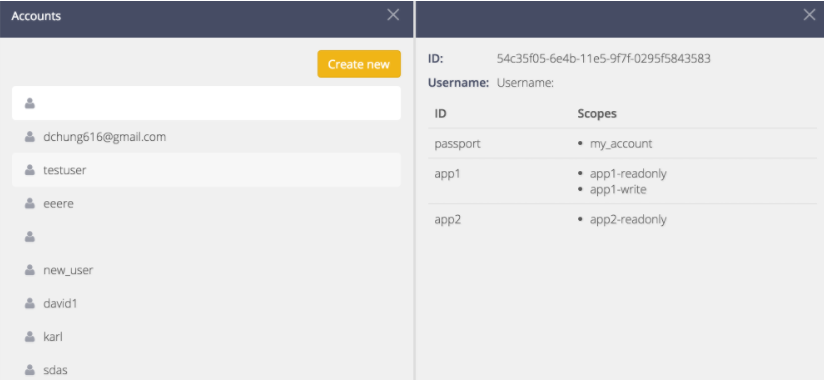
\includegraphics[scale=0.85]{manage-1.png}
	\caption{Пользователи с доступам к проекту}
	\clearpage
\end{figure}

На странице <<Console>> можно подключиться к любому серверу получив его ip. На странице появляется стандартная консоль (рисунок 7.13). Польшой пользой этого является быстрое переключение консолей для разных серверов. Для этого кликаем по нужному ip.   

\begin{figure}[h!]
\centering
	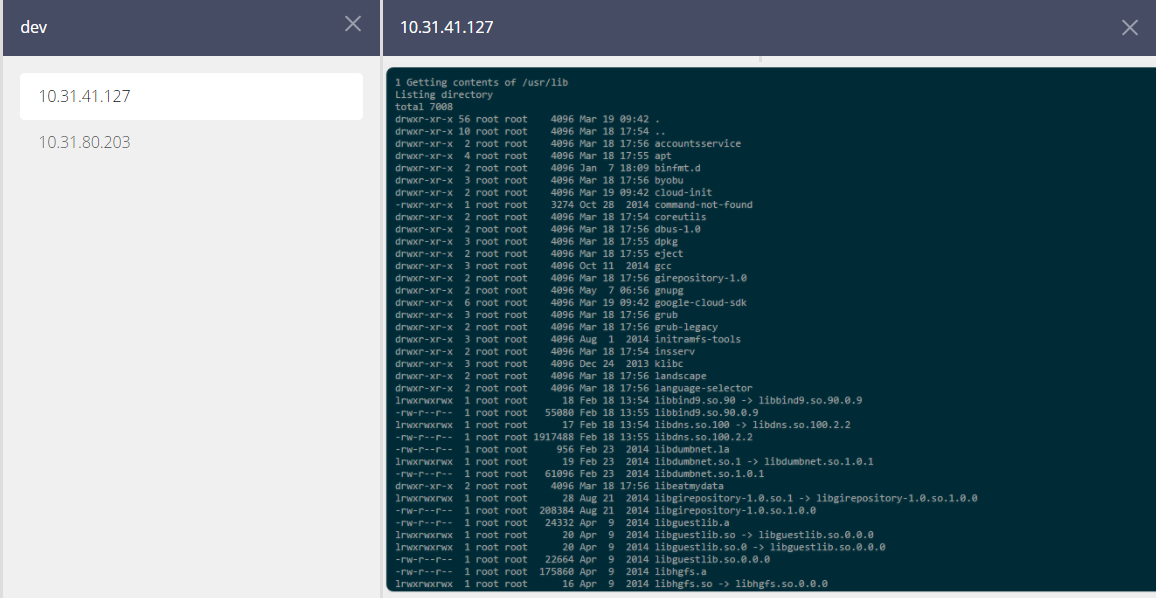
\includegraphics[scale=0.65]{console-1.png}
	\caption{Консоль}
	\clearpage
\end{figure}
